\documentclass{beamer}
\geometry{paperwidth=140mm,paperheight=105mm}
\usetheme{metropolis}           % Use metropolis theme
%\usetheme{CambridgeUS}
\title{Kolloquium zur Bachelorarbeit}
\date{07. M{\"a}rz 2018}

\institute{Universit{\"a}t Trier}

%Pseudocode
\usepackage{listings}
\usepackage{lstlinebgrd}
\lstset{
  numbers=left,
  stepnumber=1,    
  firstnumber=0,
  numberfirstline=true,
extendedchars=true, literate=%
    {Ä}{{\"A}}1%
    {Ö}{{\"O}}1%
    {Ü}{{\"U}}1%
    {ä}{{\"a}}1%
    {ö}{{\"o}}1%
    {ü}{{\"u}}1%
    {ß}{{\ss}}1%
}


%Footer
\setbeamertemplate{footline}
{
  \leavevmode%
  \hbox{%
  \begin{beamercolorbox}[wd=.4\paperwidth,ht=2.25ex,dp=1ex,center]{author in head/foot}%
    \usebeamerfont{author in head/foot}Benedikt L{\"u}ken-Winkels
  \end{beamercolorbox}%
  \begin{beamercolorbox}[wd=.6\paperwidth,ht=2.25ex,dp=1ex,center]{title in head/foot}%
    \usebeamerfont{title in head/foot}\insertshorttitle\hspace*{3em}
    \insertframenumber{} / \inserttotalframenumber\hspace*{1ex}
  \end{beamercolorbox}}%
  \vskip0pt%
}

%Mathematikumgebungen
\usepackage{amsmath,amsthm,amssymb}
\usepackage{ngerman}
\usepackage[utf8]{inputenc}
\graphicspath{{img/}}

%Farbe für Block
\definecolor{amber}{rgb}{1.0, 0.75, 0.0}
\setbeamercolor{block title}{use=text,
    fg=amber,
    bg=gray}
\setbeamercolor{block body}{use={block title , text},
    fg=text.fg,
    bg=lightgray}
    
\makeatletter    
    
\mode<presentation>{}

\begin{document}

\setbeamercovered{transparent}
\author{%
\begin{tabular}{l l} 
Referent:   & Benedikt L{\"u}ken-Winkels \\[1ex] 
Pr{\"u}fer:  & Prof. Dr. Henning Fernau\\
             & Prof. Dr.  Stefan N{\"a}her
\end{tabular}}


\maketitle
\section{Knotenüberdeckungsproblem}
\begin{frame}{Knotenüberdeckungsproblem - Definition}
\begin{block}{Knotenüberdeckung}
EINGABE: $\ Graph\ G=(V,E),\ positive\ Integer\ k\leq |V|$\\
AUSGABE: $\ S\subseteq V\ mit\ |S|\leq k,$ \textit{sodass\ jede\ Kante\ aus\ E\ einen\ Endpunkt\ in\ S\ hat.}
\end{block}			
		
\end{frame}
\section{Graphreduktion}
\begin{frame}{}
\end{frame}
  
\section{Einfache Reduktionsregeln}
\begin{frame}{Einfache Regeln}
\begin{block}{$Graph\ G=(V,E),\ Integer\ k$}\pause
\begin{enumerate}
\item $v \in V$ hat keine Kanten $\Rightarrow V = V \setminus v$ (Grad$_{0}$-Regel) \pause
\item $v \in V$ hat genau eine Kante $\Rightarrow V = V \setminus (v \cup N(v)); k = k-1 $ (Grad$_{1}$-Regel) \pause
\item $v \in V$ hat mehr als $k$ Kanten $\Rightarrow V = V \setminus (v); k = k-1 $ (Buss-Regel) \pause

\end{enumerate}
\end{block}
\end{frame}

\begin{frame}{Grad$_{1}$ - Ergebnisse}
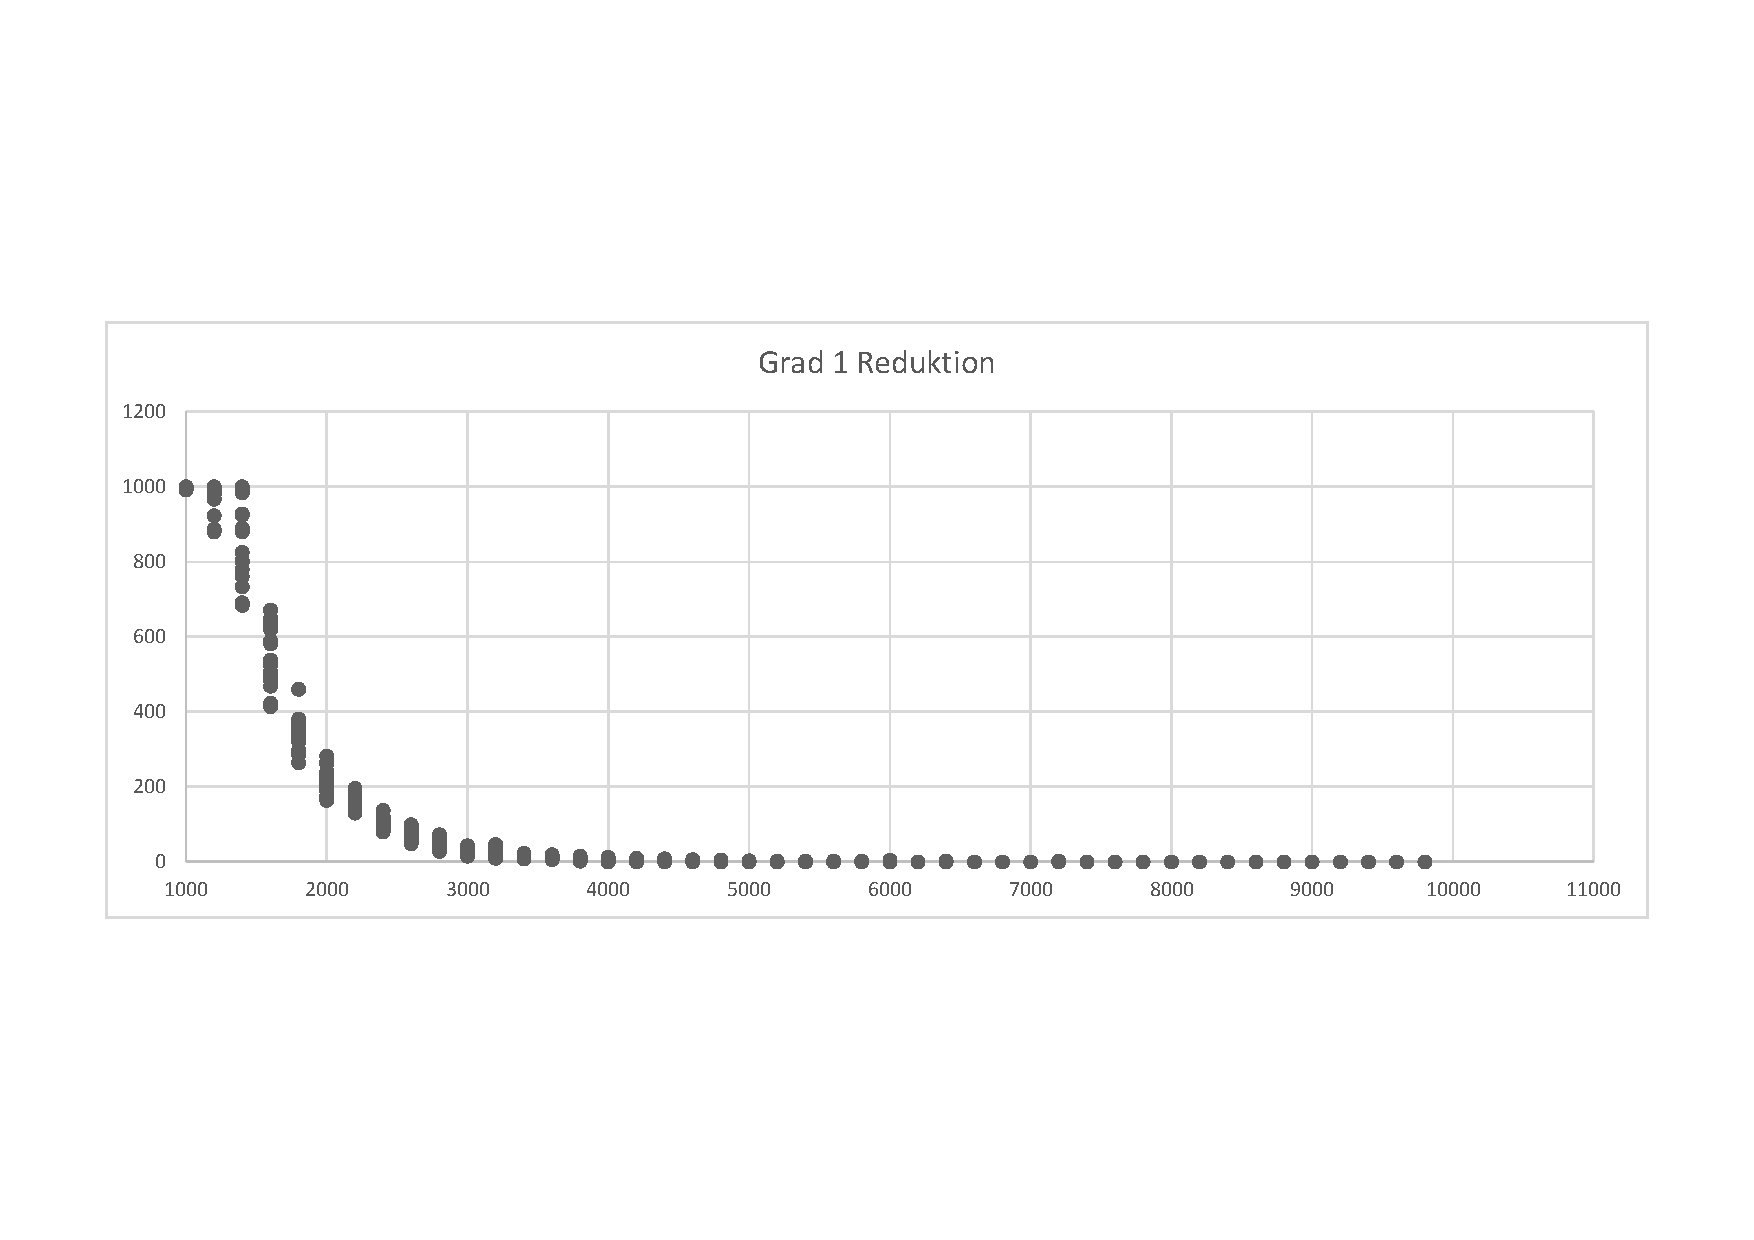
\includegraphics[scale= .4]{analysisOne.pdf} 
\end{frame}

\section{Kronenregel}
\begin{frame}[fragile]
\frametitle{Kronenregel - Algorithmus}
\begin{lstlisting}[mathescape=true, escapechar = !,basicstyle=\ttfamily\scriptsize]
$G = (V, E)$!\pause!
$M_{1}$ := Maximal Matching von $G$!\pause!
  $M_{1} := \emptyset$
  $\forall e \in$ E:	!\pause!
    $M_{1} = M_{1} \cup e$ !\pause!
    Entferne $e$ und $N(e)$ aus der weiteren Betrachtung!\pause!
$O$ := nicht gepaarte Knoten in $M_{1}$!\pause!
$M_{2}$ := Maxmimum Matching von $B = (O, N(O), \{ uv| u \in O \wedge v \in N(O)\}) $!\pause!
$I$  := nicht gepaarte Knoten aus $O$ in $M_{2}$!\pause!
$I'  := \emptyset$!\pause!
while $I' \neq I$!\pause!
  $I' := I$!\pause!
  $H:= N(I)$!\pause!
  $I := I \cup \{\forall u \in O|\exists v\in H (uv \in M_{2})\}$!\pause!
Entferne $N(I)$ aus $G$!\pause!
\end{lstlisting}
\end{frame}

\begin{frame}[fragile]
\frametitle{Kronenregel - Laufzeit}
\begin{lstlisting}[mathescape=true, escapechar = !,basicstyle=\ttfamily\scriptsize]
$G = (V, E)$
$M_{1}$ := Maximal Matching von $G$
  $M_{1} := \emptyset$
  $\forall e \in$ E:
    $M_{1} = M_{1} \cup e$
    Entferne $e$ und $N(e)$ aus der weiteren Betrachtung
$O$ := nicht gepaarte Knoten in $M_{1}$
$M_{2}$ := Maxmimum Matching von $B = (O, N(O), \{ uv| u \in O \wedge v \in N(O)\}) $
$I$  := nicht gepaarte Knoten aus $O$ in $M_{2}$
$I'  := \emptyset$
while $I' \neq I$
  $I' := I$
  $H:= N(I)$
  $I := I \cup \{\forall u \in O|\exists v\in H (uv \in M_{2})\}$
Entferne $N(I)$ aus $G$
\end{lstlisting}
\only<1>{Zeilen 1-5: $m \cdot d$}
\only<2>{Zeile 6: $n$}
\only<3>{Zeile 7(1): $\frac{(n-2k) d}{2}$}
\only<4>{Zeile 7(1): $\sqrt{n-2k} \cdot m $ (LEDA:mcb\_matching, Hopcroft und Karp) }
\only<5>{Zeile 8:  }


\end{frame}


\begin{frame}{Kronenegel - Laufzeit}
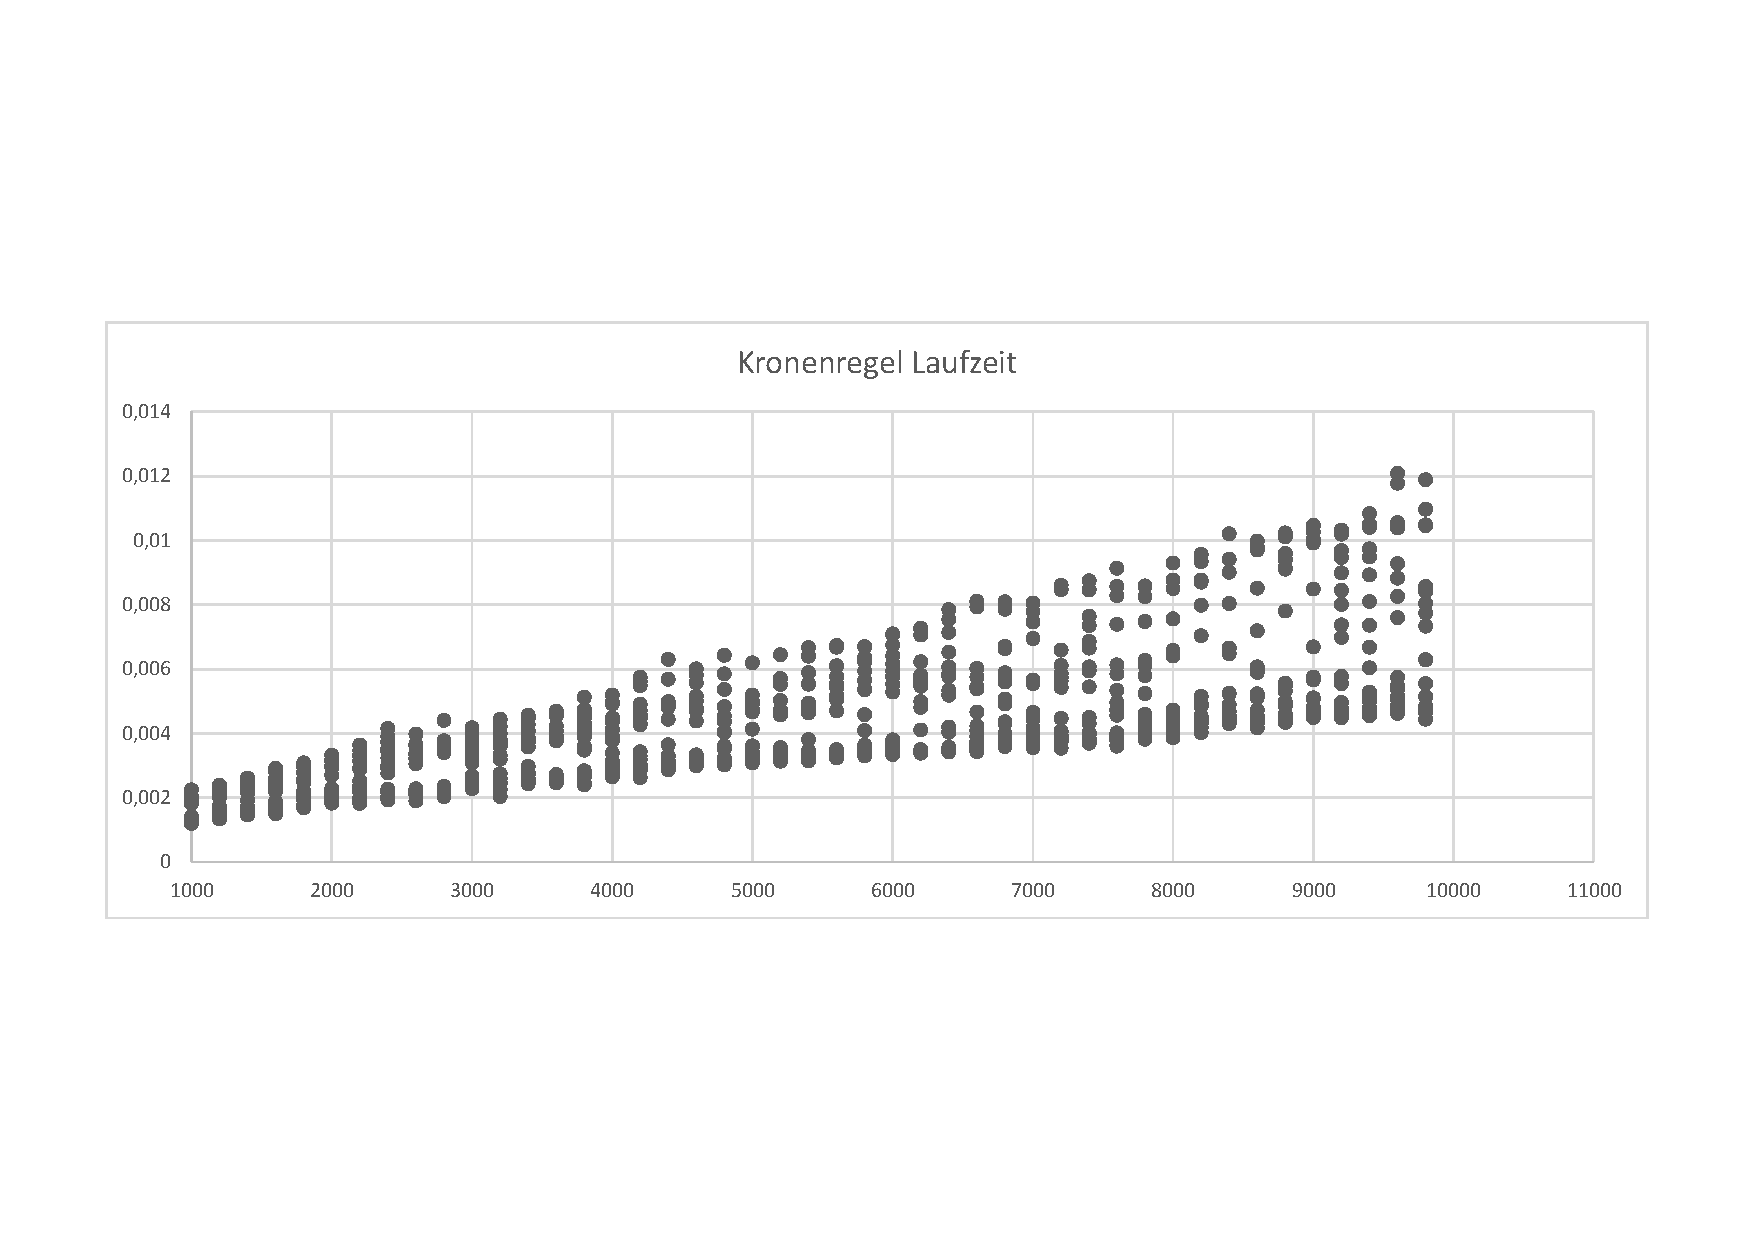
\includegraphics[scale= .4]{analysis1000_CrownNormal_runtime.pdf} 
\end{frame}

\begin{frame}{Kronenregel - Ergebnisse}
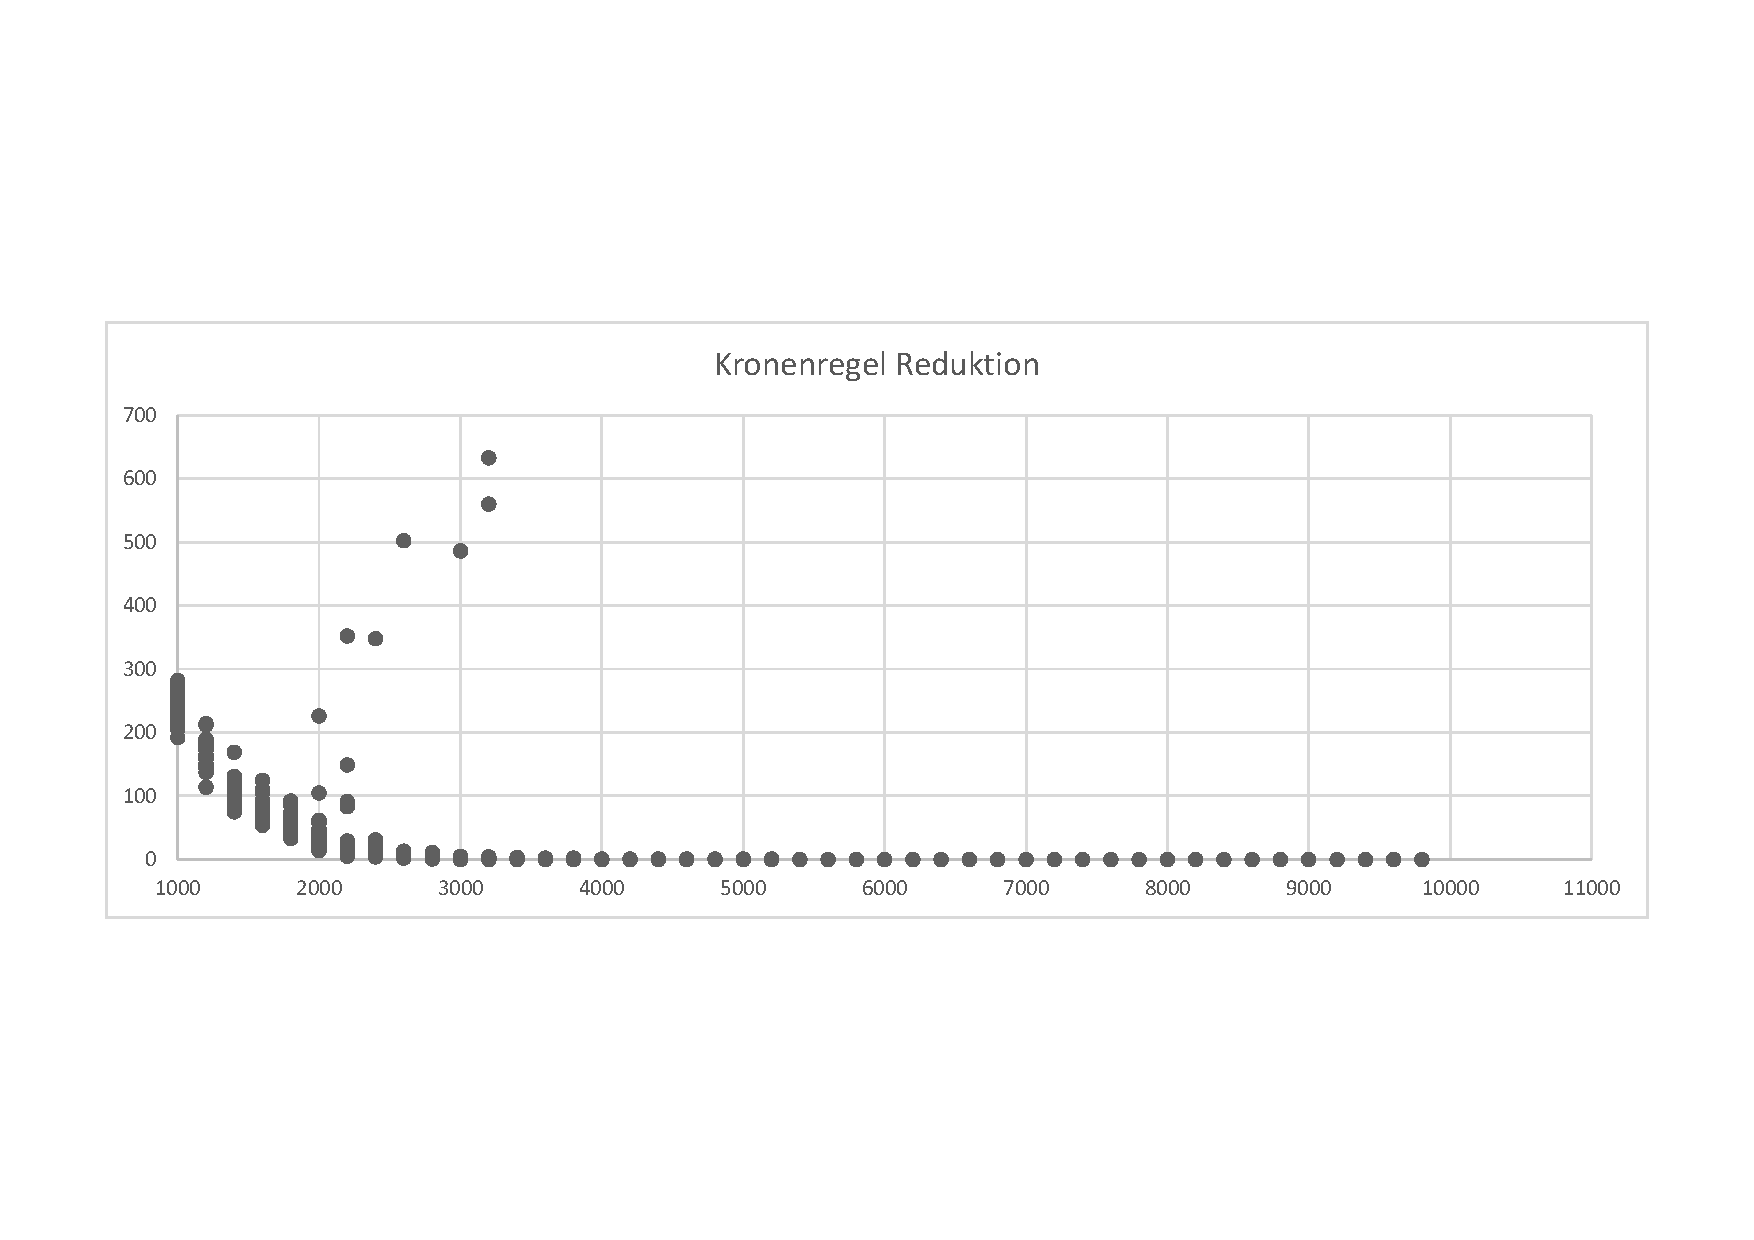
\includegraphics[scale= .4]{analysisCrown.pdf} 
\end{frame}

\section{Nemhauser-Trotter-Regel}
	
\begin{frame}{Nemhauser-Trotter-Regel}
\begin{block}{Nemhauser-Trotter-Theorem}
$\textit{Für einen Graphen}\ G=(V,E)\textit{ können zwei disjunkte Mengen}$\\ $\ C_{0}\ und\ V_{0} \textit{ gefunden werden, sodass}$
\begin{enumerate}[<+->]
\item $C_{0}$ \textit{ in einer minimalen Knotenüberdeckung} \\ 
\textit{von G enthalten ist,}
\item \textit{der Teilgraph }$G[V_{0}]$ \textit{eine Knotenüberdeckung}\\
\textit{der Größe} $\leq |V_{0}| / 2$ \textit{ hat,}
\item \textit{und} $VC(G) = VC(G[V_{0}])\cup C_{0}$ \textit{ gilt.}
\end{enumerate}

\end{block}
\end{frame}
	
\begin{frame}[fragile]
\frametitle{NT-Regel - Algorithmus}
\begin{lstlisting}[mathescape = true, basicstyle=\ttfamily, escapechar = !]
$G = (V, E)$!\pause!
Bipartiden Graphen erstellen $B = (V, V', E')$
  mit $E':= \{\{x,y'\}, \{x', y\} | \{x,y\} \in E\}$!\pause!
Maximum Matching $M$ von $B$ bestimmen!\pause!
$C_{B}:= VC(B)$!\pause!
$C_{0}:= \{x \in V\ |\ x \in C_{B}\ und\ x' \in C_{B} \}$!\pause!
$V_{0}:= \{x \in V\ |\ entweder\ x \in C_{B}\ oder\ x' \in C_{B} \}$
\end{lstlisting}

\end{frame}

\begin{frame}[fragile]
\frametitle{NT-Regel - Laufzeit}
\begin{lstlisting}[mathescape = true, basicstyle=\ttfamily]
$G = (V, E)$
Bipartiden Graphen erstellen $B = (V, V', E')$ 
  mit $E':= \{\{x,y'\}, \{x', y\} | \{x,y\} \in E\}$ 
Maximum Matching $M$ von $B$ bestimmen 
$C_{B}:= VC(B)$ 
$C_{0}:= \{x \in V\ |\ x \in C_{B}\ und\ x' \in C_{B} \}$ 
$V_{0}:= \{x \in V\ |\ entweder\ x \in C_{B}\ oder\ x' \in C_{B} \}$ 
\end{lstlisting}
\only<1>{Zeilen 1-2: $n \cdot 2d$}
\only<2>{Zeilen 3-4: $\sqrt{n} \cdot m$ (LEDA:mcb\_matching, Hopcroft und Karp)}
\only<3>{Zeilen 5-6: $2n + k \cdot d$}
\only<4>{$n \cdot 2d + \sqrt{n} \cdot m + 2n + k \cdot d$}
\only<5>{$n \cdot 2d + \sqrt{n} \cdot m + 2n + k \cdot d \Rightarrow O(n + \sqrt{n} \cdot m)$}
\end{frame}
\begin{frame}{NT-Regel - Laufzeit}
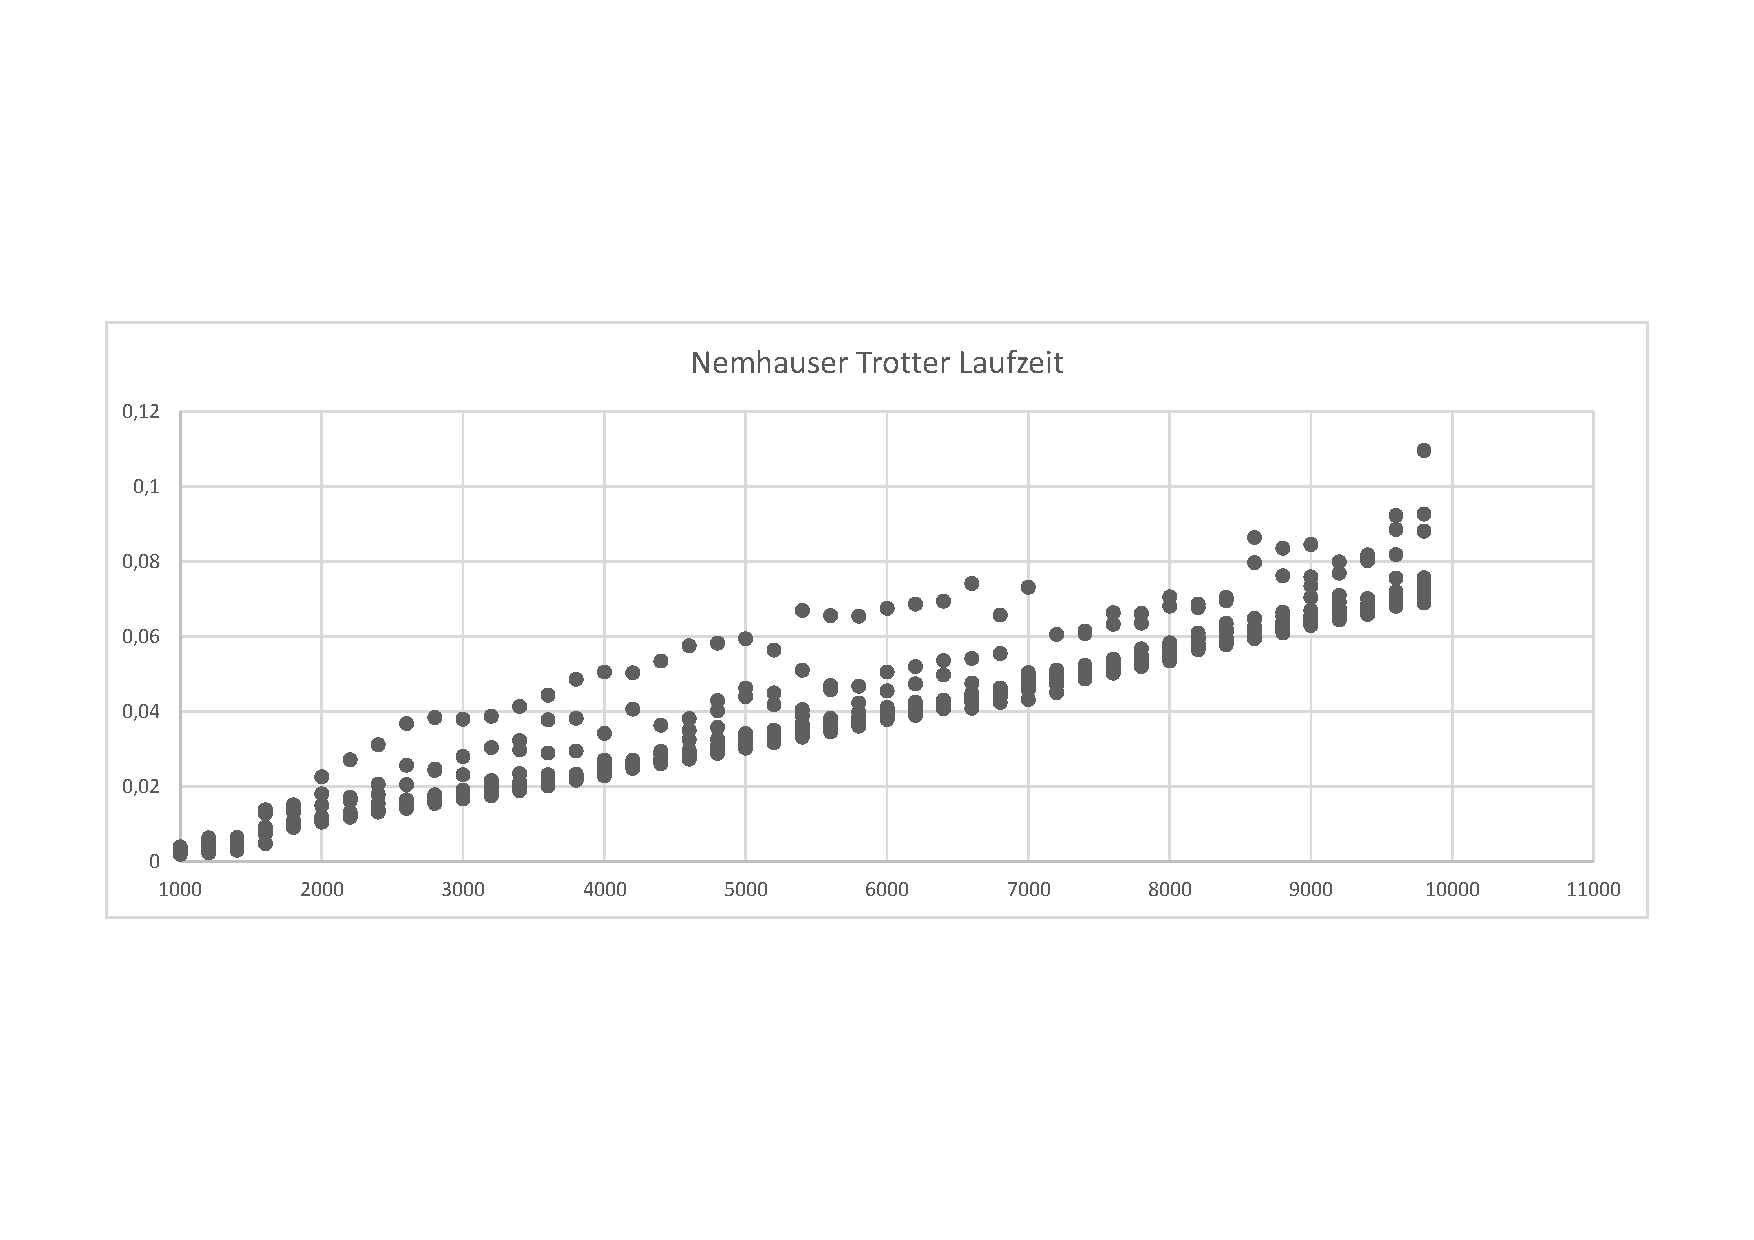
\includegraphics[scale= .4]{analysis1000_TrottNormal_runtime.pdf} 
\end{frame}
\begin{frame}{NT-Regel - Ergebnisse}
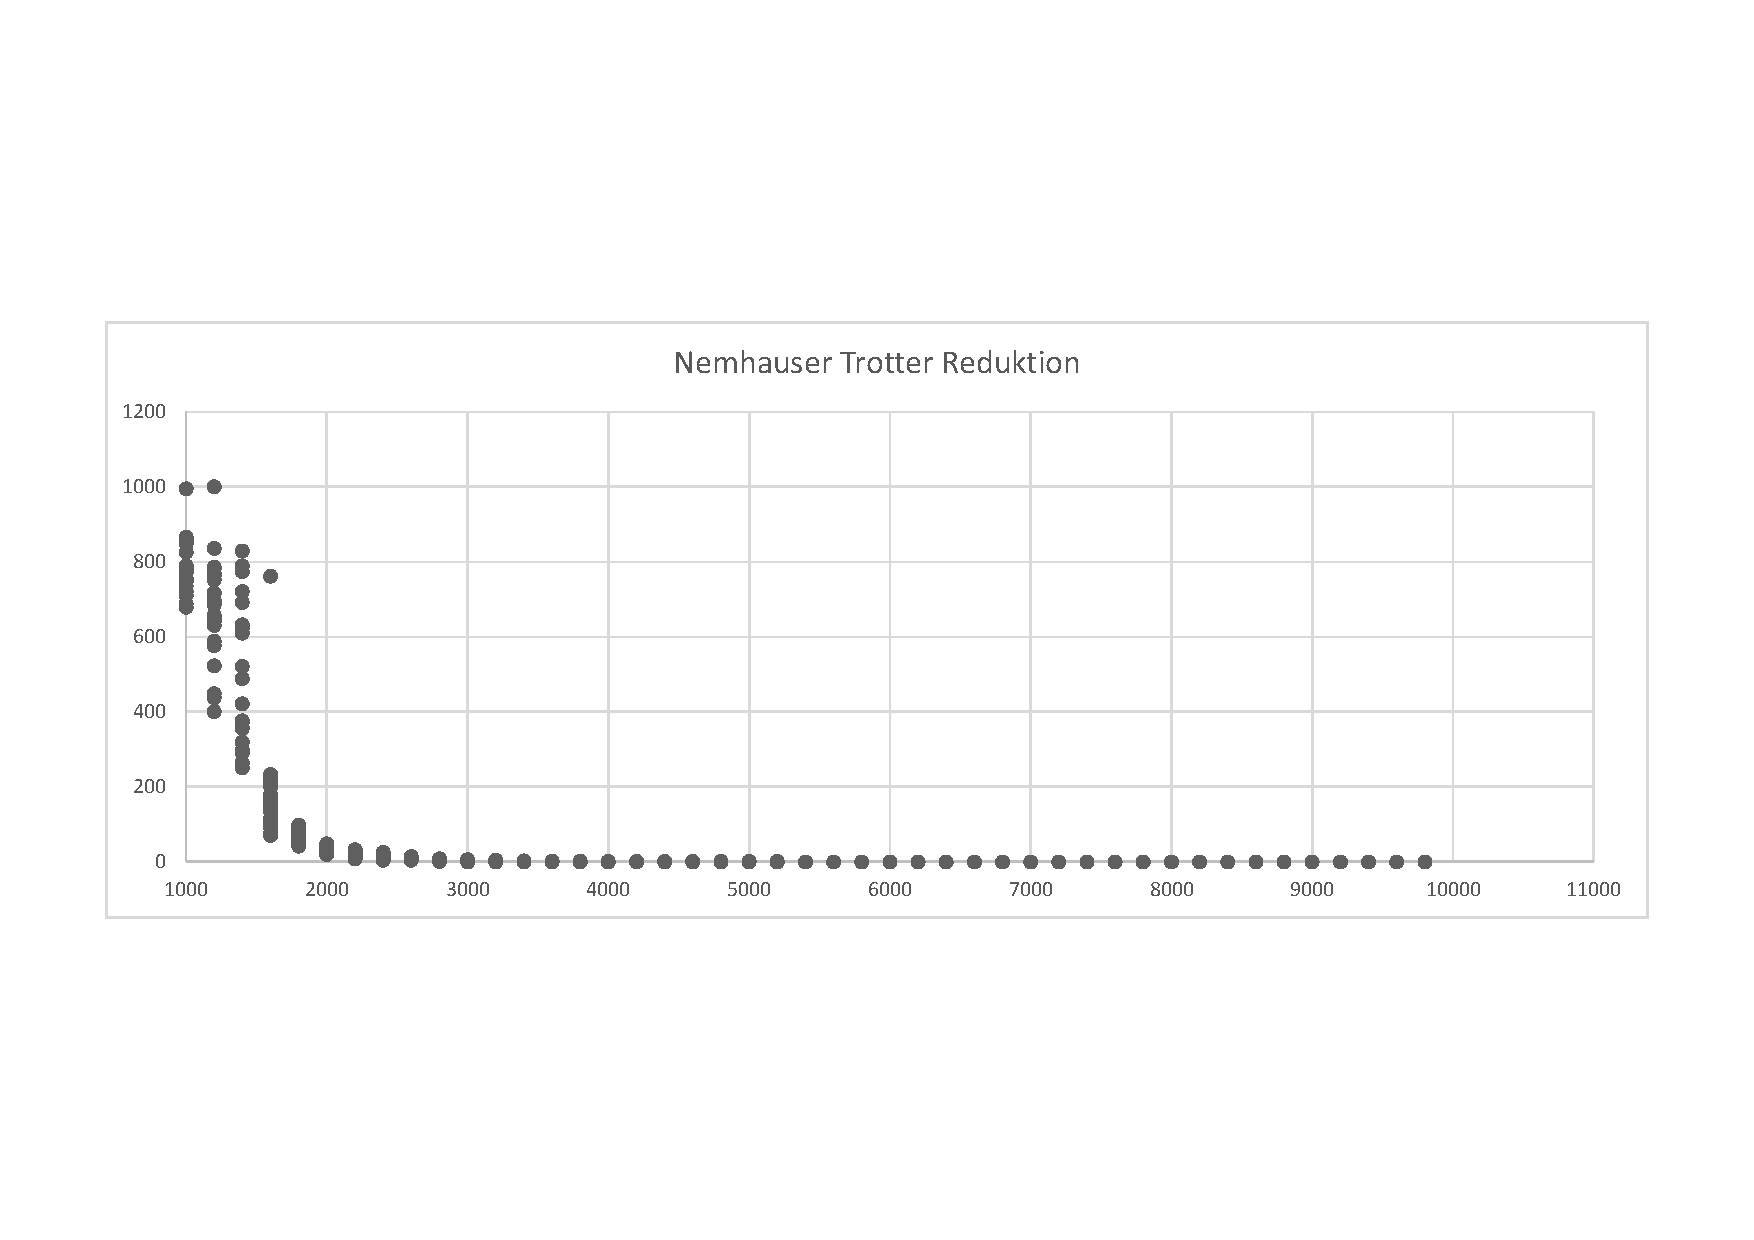
\includegraphics[scale= .4]{analysisTrott.pdf} 
\end{frame}

\section{Vergleich}
\begin{frame}{}
\end{frame}
\section{Anwendung}
\begin{frame}{}
\begin{table}[htbp]
\caption{Anwendung kombinierter Reduktionsregeln\label{tab:kombination}}
\vspace*{1em}
\centering

\bgroup
\def\arraystretch{1.3}%  1 is the default, change whatever you need
\tiny
\begin{tabular}[c]{l|l|l|l|l}

	
	\multicolumn{1}{c|}{\textbf{Kombination}} &
	\multicolumn{1}{c|}{\textbf{Anwendungen$_{1}$}} &
	\multicolumn{1}{c|}{\textbf{Anwendungen$_{2}$}} &
	\multicolumn{1}{c|}{\textbf{Anwendungen$_{3}$}} & 
	\multicolumn{1}{c}{\textbf{Reduktion}} \\
	\hline

	K - G$_{1}$ & 3.63 & 4.3 & - &331.8\\
	G$_{1}$ - K & 4.37 & 3.22 & - &331.17\\
	K - NT & 0.8 & 0.38 & - & 68.28 \\
	NT - K & 0.45 & 0.56 & - & 68.6\\
	G$_{1}$ - NT & 1.33 & 0.017 & - & 99.87\\
	NT - G$_{1}$ & 0.28 & 1.13 & - & 99.87\\
	K  - G$_{1}$ - NT & 3.61 & 4.29 & 0.11 & 334.67 \\
	K - NT - G$_{1}$ & 3.6 & 0.87 & 3.39 & 334.83 \\
	G$_{1}$ - NT - K & 4.36 & 0.12 & 3.2 & 334.17 \\
	G$_{1}$ - K - NT & 3.61 & 3.2 & 0.65 & 334.16 \\
	NT - K - G$_{1}$ & 0.39 & 3.44 & 4.03 & 335.2 \\
	NT - G$_{1}$ - K & 0.91 & 3.42 & 3.2 & 334.16 \\

	
\end{tabular}

\egroup

\end{table}
\end{frame}
	
\section{Implementierung}
\begin{frame}{}
\end{frame}

\section{Fazit}
\begin{frame}{}
\end{frame}
  
\end{document}